\documentclass[fleqn]{article}
\usepackage{geometry}
\usepackage{amsmath}
\usepackage{amsthm}
\usepackage{graphicx}
\usepackage{caption}
\usepackage[utf8]{inputenc}


%%%%%%%% SUB-FIGURE PACKAGE
\usepackage{subcaption}

%%%%%%%% MULTI-COLUMNS PACKAGE
\usepackage{multicol}

%%%%%%%% PERSONAL COMMANDS
\usepackage{amssymb}

%%%% Important sets
\renewcommand{\O}{\mathbb{O}}
\newcommand{\N}{\mathbb{N}}
\newcommand{\Z}{{\mathbb{Z}}}
\newcommand{\Q}{{\mathbb{Q}}}
\newcommand{\R}{{\mathbb{R}}}

%%%% Usual operations
\newcommand{\pow}[2]{#1^{#2}}
\newcommand{\expp}[1]{e^{#1}}
\newcommand{\fst}{\mathrm{fst}}
\newcommand{\snd}{\mathrm{snd}}

%%%% Lambda Calculus
\newcommand{\dneq}{\,\, \# \,\,}
\newcommand{\prm}[1]{\pmb{\mathrm{#1}}}
\renewcommand{\S}{\prm{S}}
\newcommand{\I}{\prm{I}}
\newcommand{\K}{\prm{K}}
\newcommand{\ch}[1]{\ulcorner #1 \urcorner}

%%%% Ordinal Lambda Calculus
\newcommand{\ordAlph}{\Sigma_{\text{Ord}}}
\newcommand{\termOrd}{\text{Term}_\text{Ord}}
\newcommand{\fl}{\mathrm{fl}}
\newcommand{\sk}{\mathrm{sk}}

%% Superscript to the left
% https://latex.org/forum/viewtopic.php?t=455
\usepackage{tensor}
\newcommand{\app}[3]{\tensor*[^{#1}]{\left(#2, #3\right)}{}}

%%%% Make optional parameter
% https://bit.ly/3jVGRwQ
\usepackage{xparse}

%%%% Statistics
\NewDocumentCommand{\E}{o m}{
  \IfNoValueTF{#1}
  {\mathbb{E}\left[#2\right]}
  {\mathbb{E}^{#1}\left[ #2\right]}
}
\NewDocumentCommand{\V}{o m}{
  \IfNoValueTF{#1}
  {\mathrm{Var}\left[#2\right]}
  {\mathrm{Var}^{#1}\left[ #2\right]}
}
\RenewDocumentCommand{\P}{o o m}{
  \IfNoValueTF{#1}
  {\IfNoValueTF{#2}
    {\mathrm{P}\left(#3\right)}
    {\mathrm{P}^{#2}\left(#3\right)}}
  {\IfNoValueTF{#2}
    {\mathrm{P}_{#1}\left(#3\right)}
    {\mathrm{P}_{#1}^{#2} \left(#3\right)}}
}

%%%% Lambda Calculus
\NewDocumentCommand{\cx}{o}{
  \IfNoValueTF{#1}
  {\left[\quad\right]}
  {\left[\, #1 \,\right]}
}

%%%% Create absolute value function
% https://bit.ly/33Rkq6H
\usepackage{mathtools}
\DeclarePairedDelimiter\abs{\lvert}{\rvert}%
\DeclarePairedDelimiter\norm{\lVert}{\rVert}%
\makeatletter
\let\oldabs\abs
\def\abs{\@ifstar{\oldabs}{\oldabs*}}
%
\let\oldnorm\norm
\def\norm{\@ifstar{\oldnorm}{\oldnorm*}}
\makeatother

%%%%%%%% LOGIC TREES
\usepackage{prftree}

%%%%%%%% SPLIT EQUATIONS
% https://bit.ly/33P1OUM
\allowdisplaybreaks

%%%%%%%% FLOAT SPECIFIER
% https://bit.ly/30Wi4BC
\usepackage{float}

%%%%%%%% TO USE SHORT COMMANDS FOR VECTOR LINES
\usepackage{esvect}

%%%%%%%% ENUMERATE LABEL
% https://www.latex-tutorial.com/tutorials/lists/
\usepackage{enumitem}

%%%%%%%% DIFFERENT FONTS FOR MATH
\usepackage{mathrsfs}


%%%%%%%% MARGIN
\usepackage[left=1in, right=1in, top=0.8in, bottom=0.8in]{geometry}

%%%%%%%% NO PARAGRAPH INDENT
% https://tex.stackexchange.com/questions/27802/set-noindent-for-entire-file
\setlength\parindent{0pt}

%%%%%%%% HYPERREF PACKAGE
\usepackage{hyperref}
\hypersetup{linkcolor=blue}
\hypersetup{citecolor=blue}
\hypersetup{urlcolor=blue}
\hypersetup{colorlinks=true}

%%%%%%%% CODE RENDERING !!! UNCOMMENT IF NEEDED !!!
% Compile with flag -shell-escape
\usepackage{minted}
\usemintedstyle{vs}

%%%%%%%% EXAM PACKAGE
\usepackage{mathexam}

%%%%%%%% START DOCUMENT
\ExamClass{ANÁLISIS NUMÉRICO 2}
\ExamName{EXAMEN 3}
\ExamHead{\today}

\let\ds\displaystyle

\begin{document}
\vspace{0.3cm}
   % Information of the student
\begin{itemize}[leftmargin=6.25cm, labelsep=0.5cm]

  \item[\textit{Nombre}] \scalebox{1.2}{Juan Sebastián Cárdenas
    Rodríguez} % Name
  \item[\textit{Código}] 201710008101 % Code

\end{itemize}
\vspace{0.3cm}

% Each of the items to solve
\begin{enumerate}
  \item Pregunta.
        \begin{enumerate}
          \item Para hallar la fórmula débil, sea $v \in \mathcal{H}_{0}^{1}$.
                \begin{figure}[H]
                  \centering 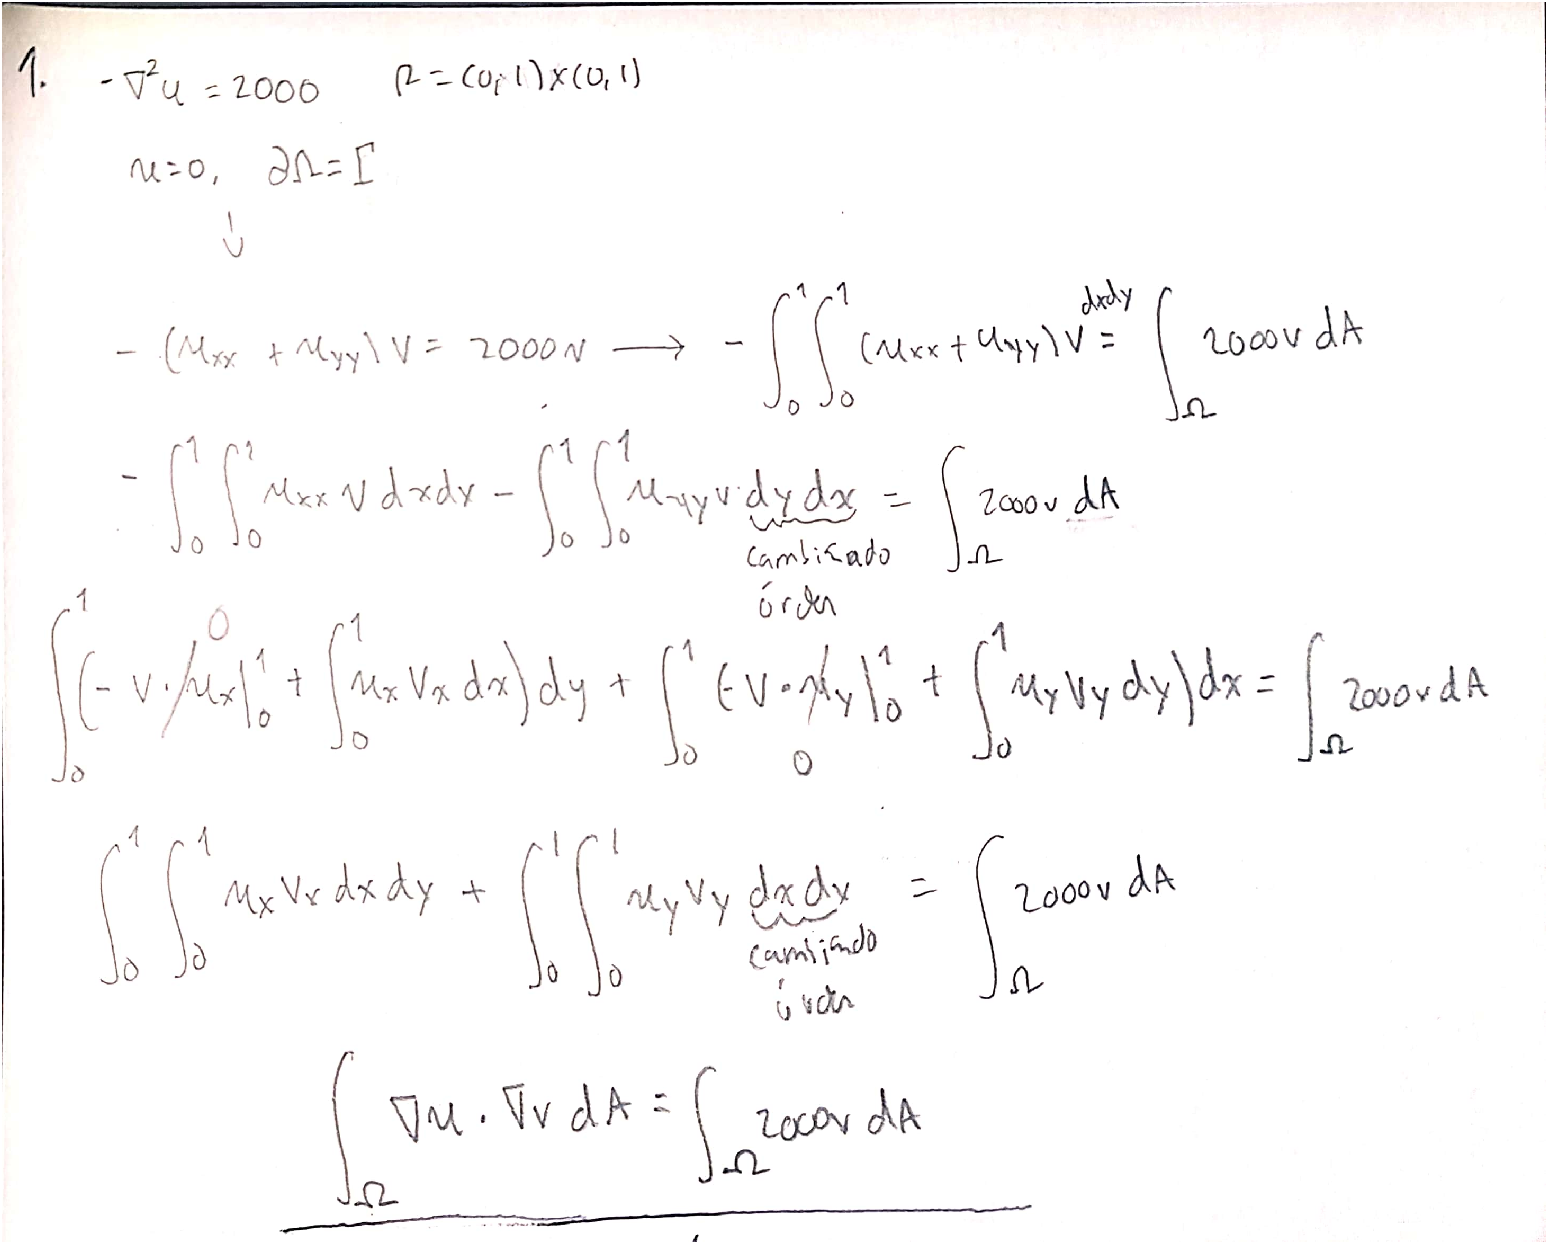
\includegraphics[scale=.5]{figs/1a}
                \end{figure}

          \item Esta aproximación, ya dada la formulación variacional, se estimó
                utilizando el paquete \texttt{FEniCS}. El código se puede
                encontrar a continuación:

                \inputminted{python}{../exercises/exam.py}
                %
                De esta manera, se encuentran dos gráficas principalmente, una
                que muestra la aproximación de $u$ para diferentes $x$ y $y$; y
                la otra que muestra la proyección de $u$ en el plano
                duodimensional. Ambas gráficas se pueden encontrar a
                continuación:
                %
                \begin{figure}[H]
                  \begin{subfigure}[b]{0.45\textwidth}
                    \centering 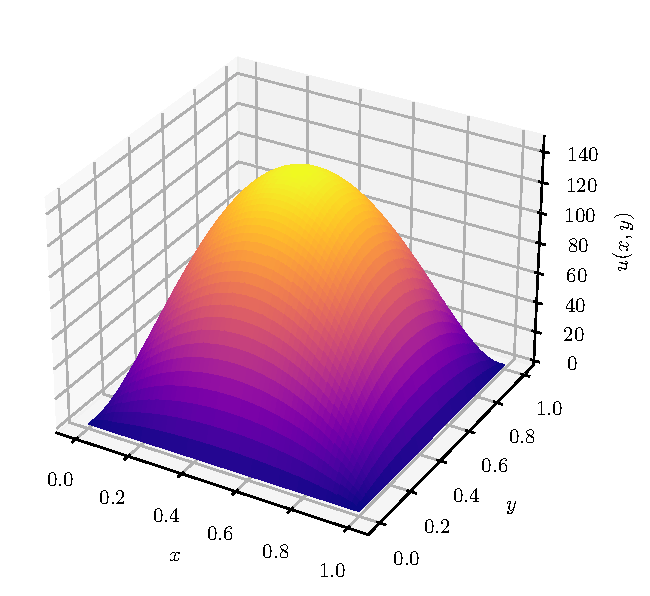
\includegraphics[scale=.7]{figs/plot3d}
                    \caption{Aproximación 3D.}
                  \end{subfigure}
                  %
                  \begin{subfigure}[b]{0.45\textwidth}
                    \centering 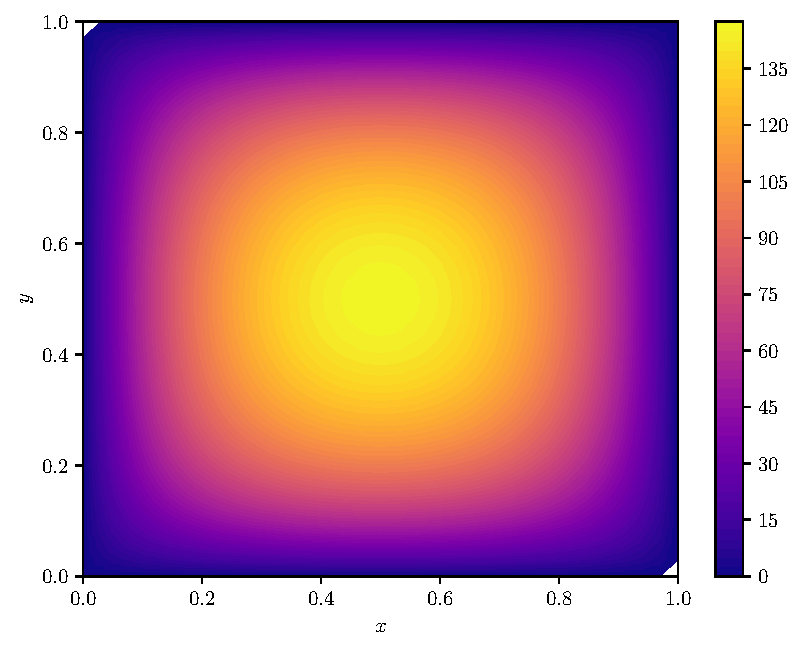
\includegraphics[scale=.5]{figs/plot2d}
                    \caption{Proyección de la aproximación 2D.}
                  \end{subfigure}
                \end{figure}
        \end{enumerate}
  \item Pregunta.
        \begin{figure}[H]
          \centering 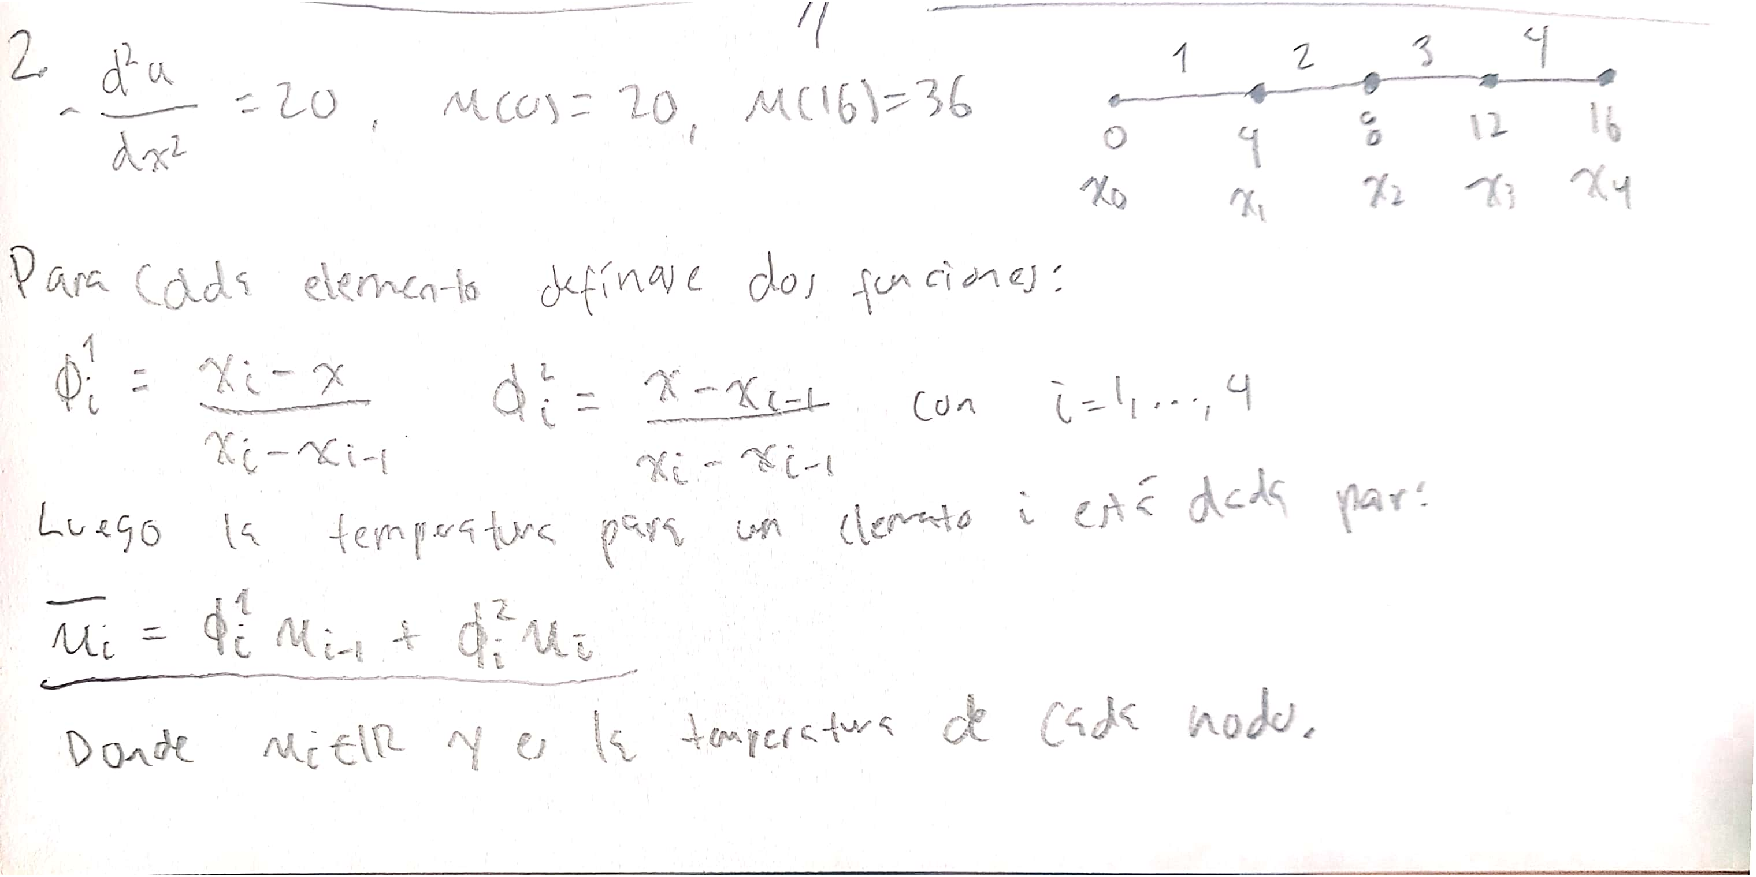
\includegraphics[scale=.3]{figs/21}
        \end{figure}
        \begin{figure}[H]
          \centering 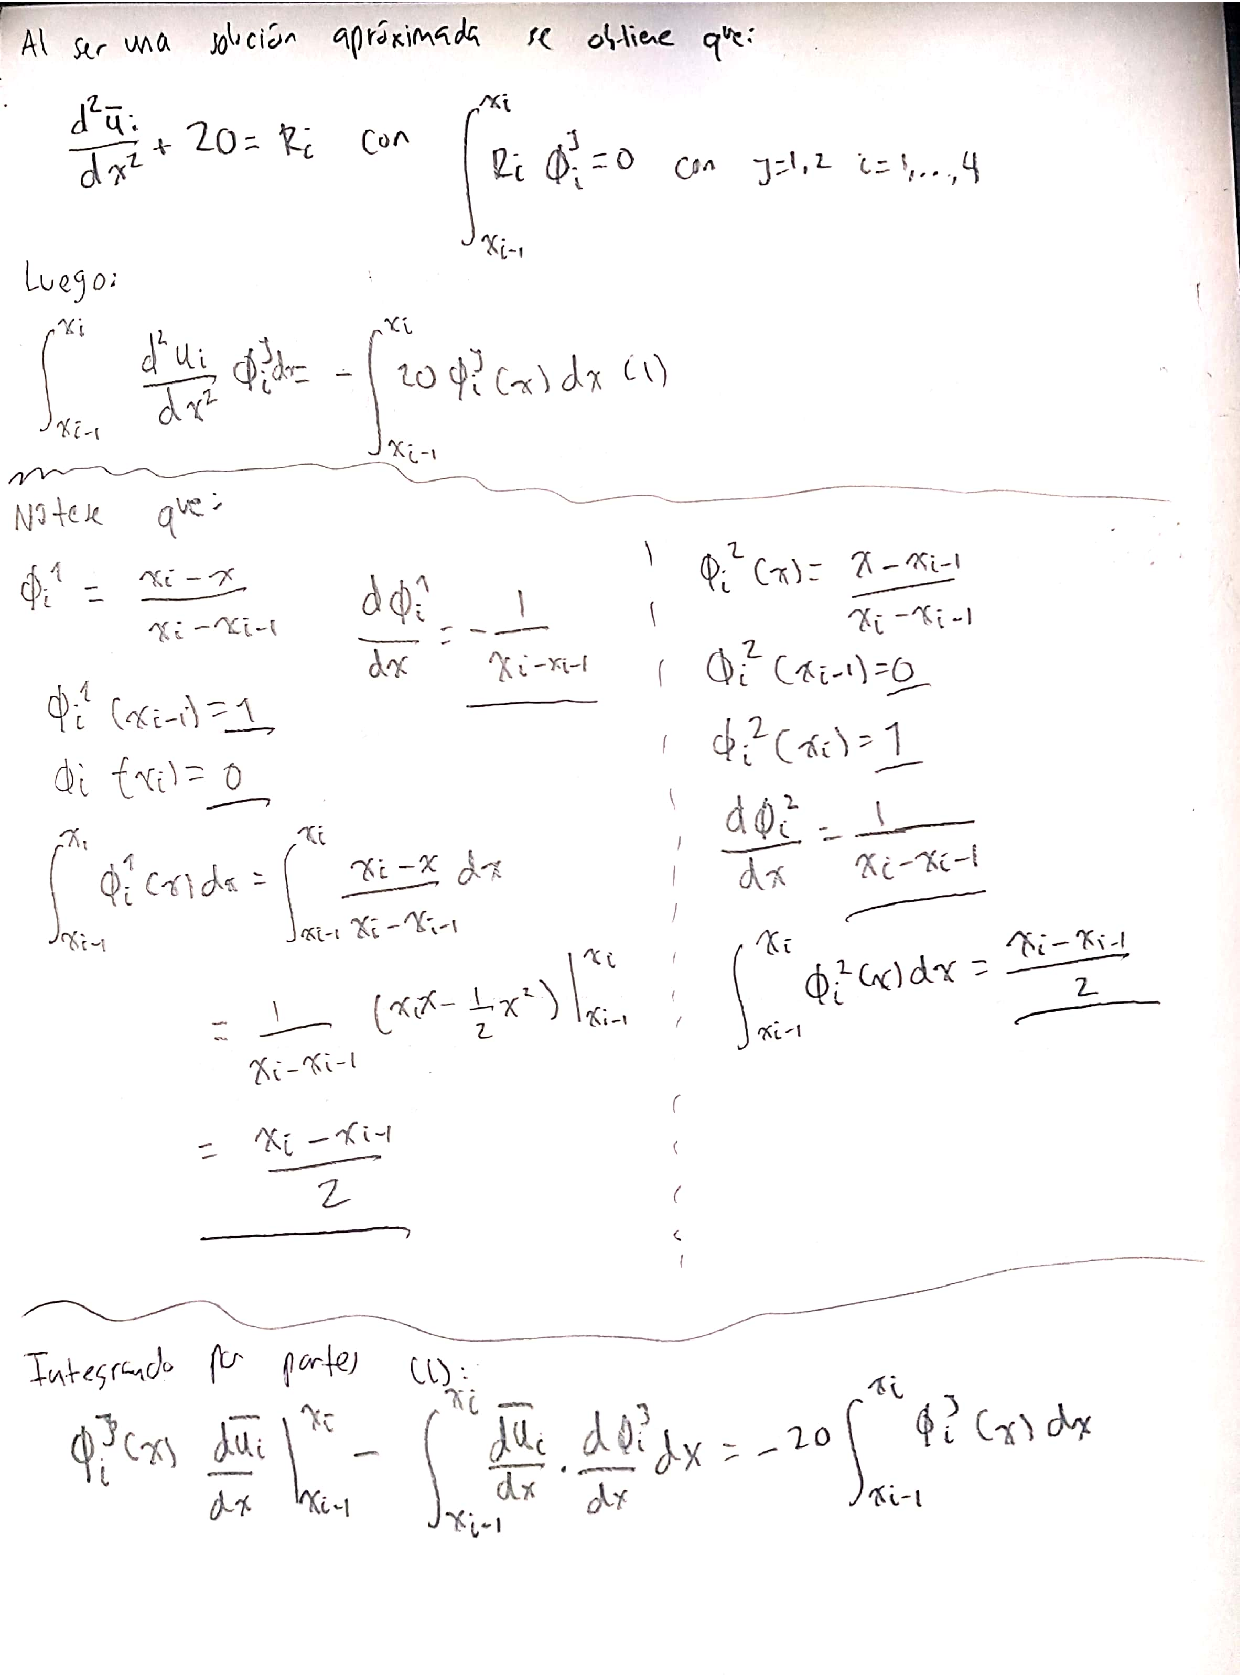
\includegraphics[scale=.8]{figs/22}
        \end{figure}
        \begin{figure}[H]
          \centering 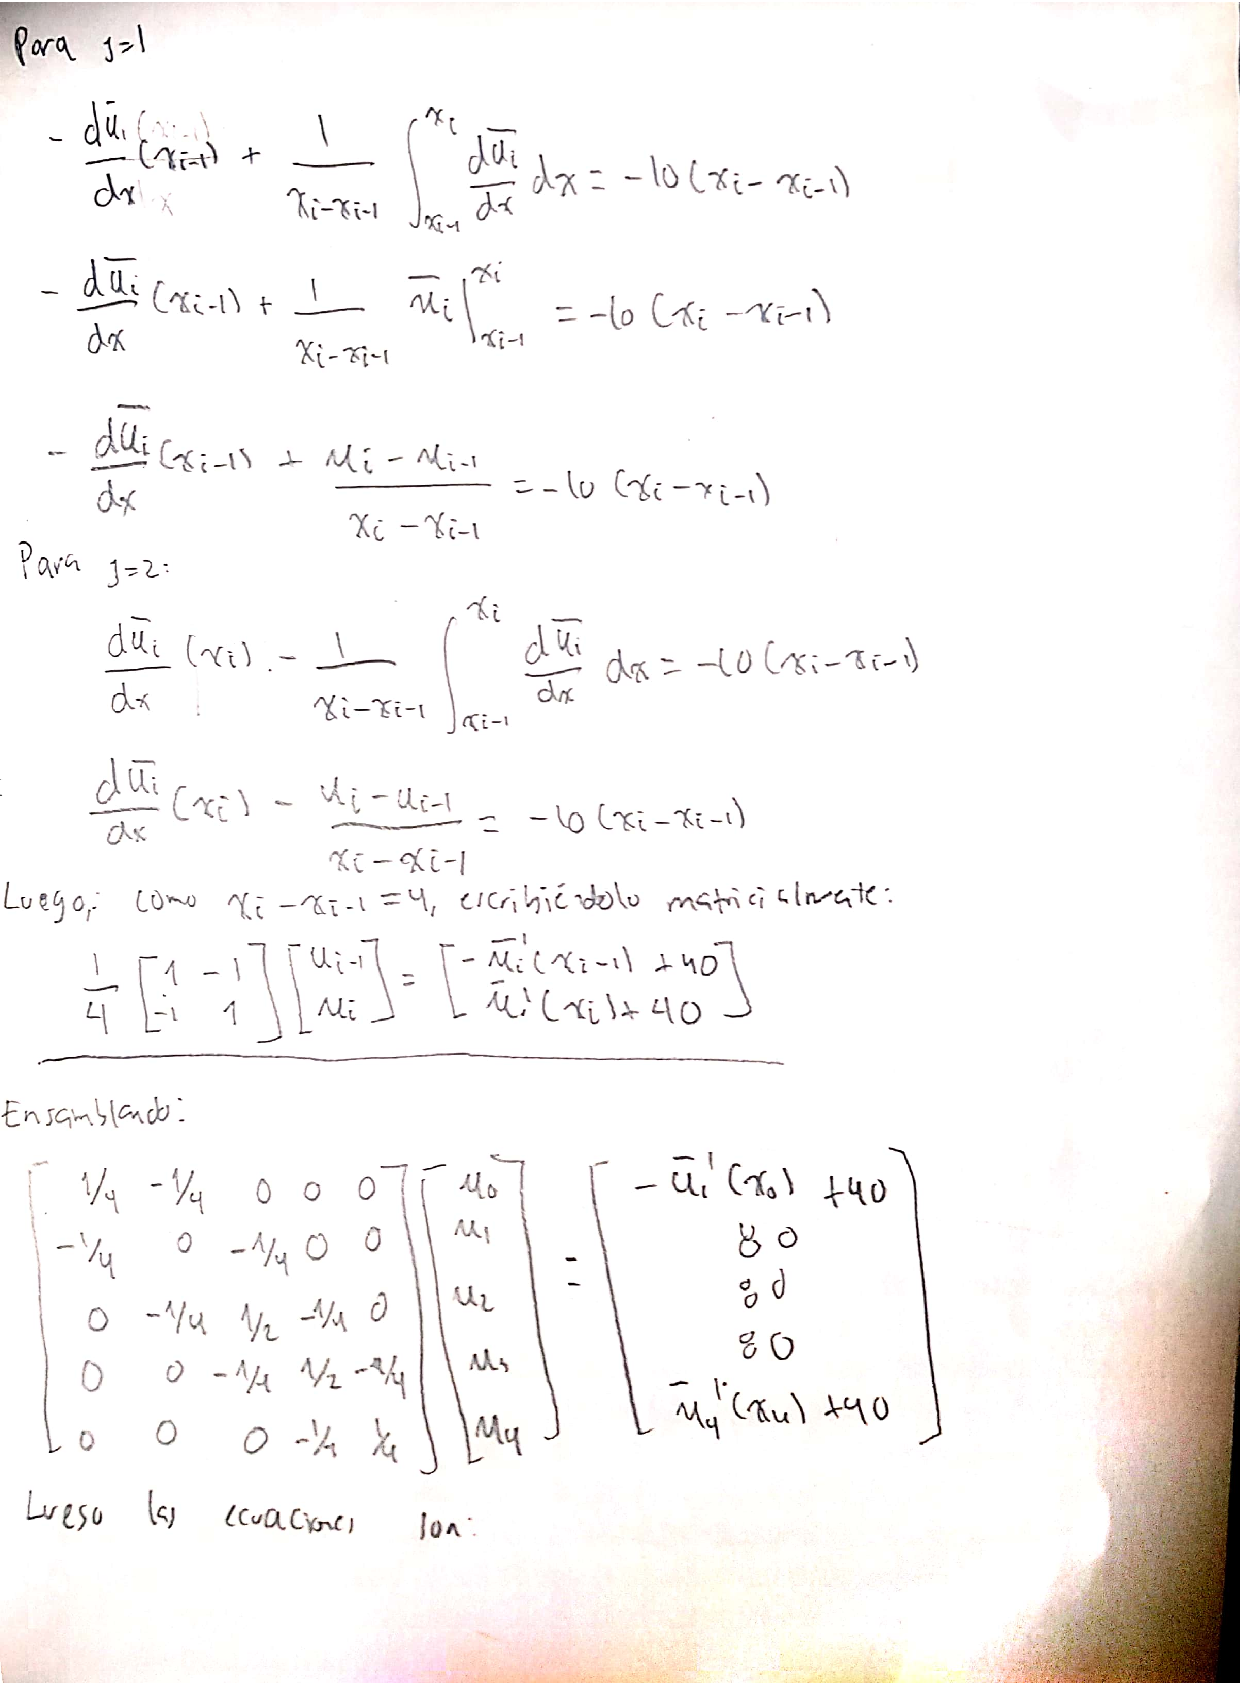
\includegraphics[scale=.8]{figs/23}
        \end{figure}
        \begin{figure}[H]
          \centering 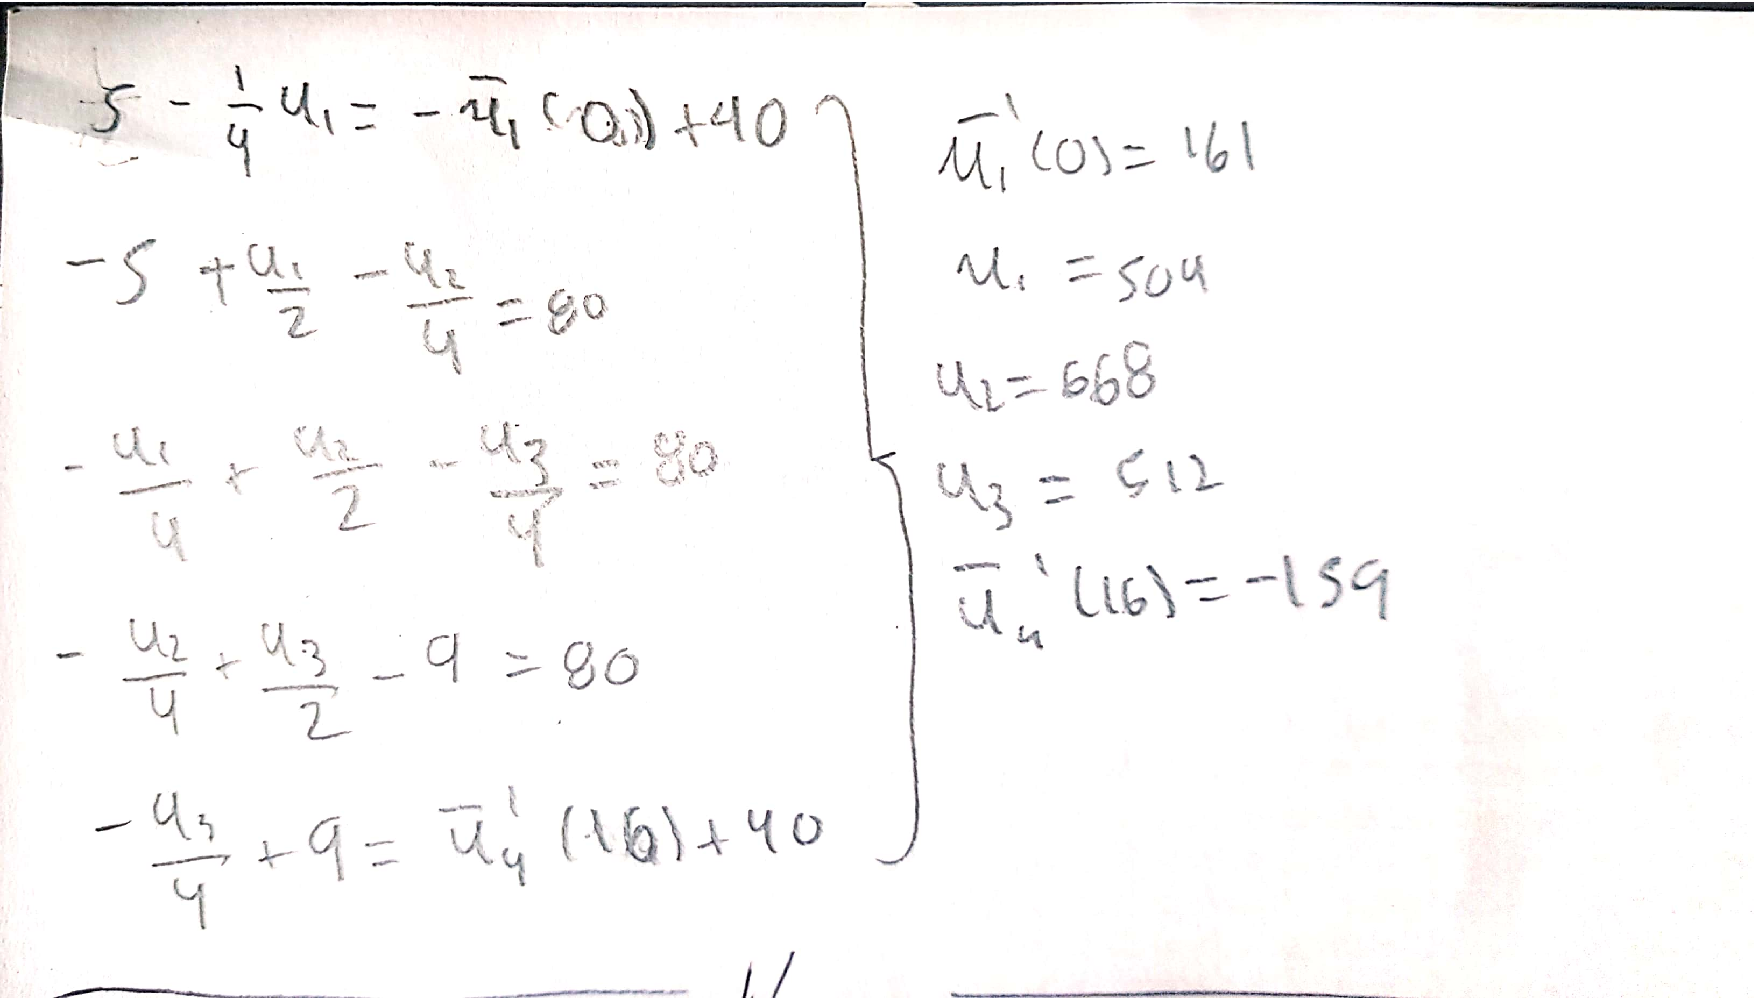
\includegraphics[scale=.3]{figs/24}
        \end{figure}
  \item Pregunta.
        \begin{figure}[H]
          \centering 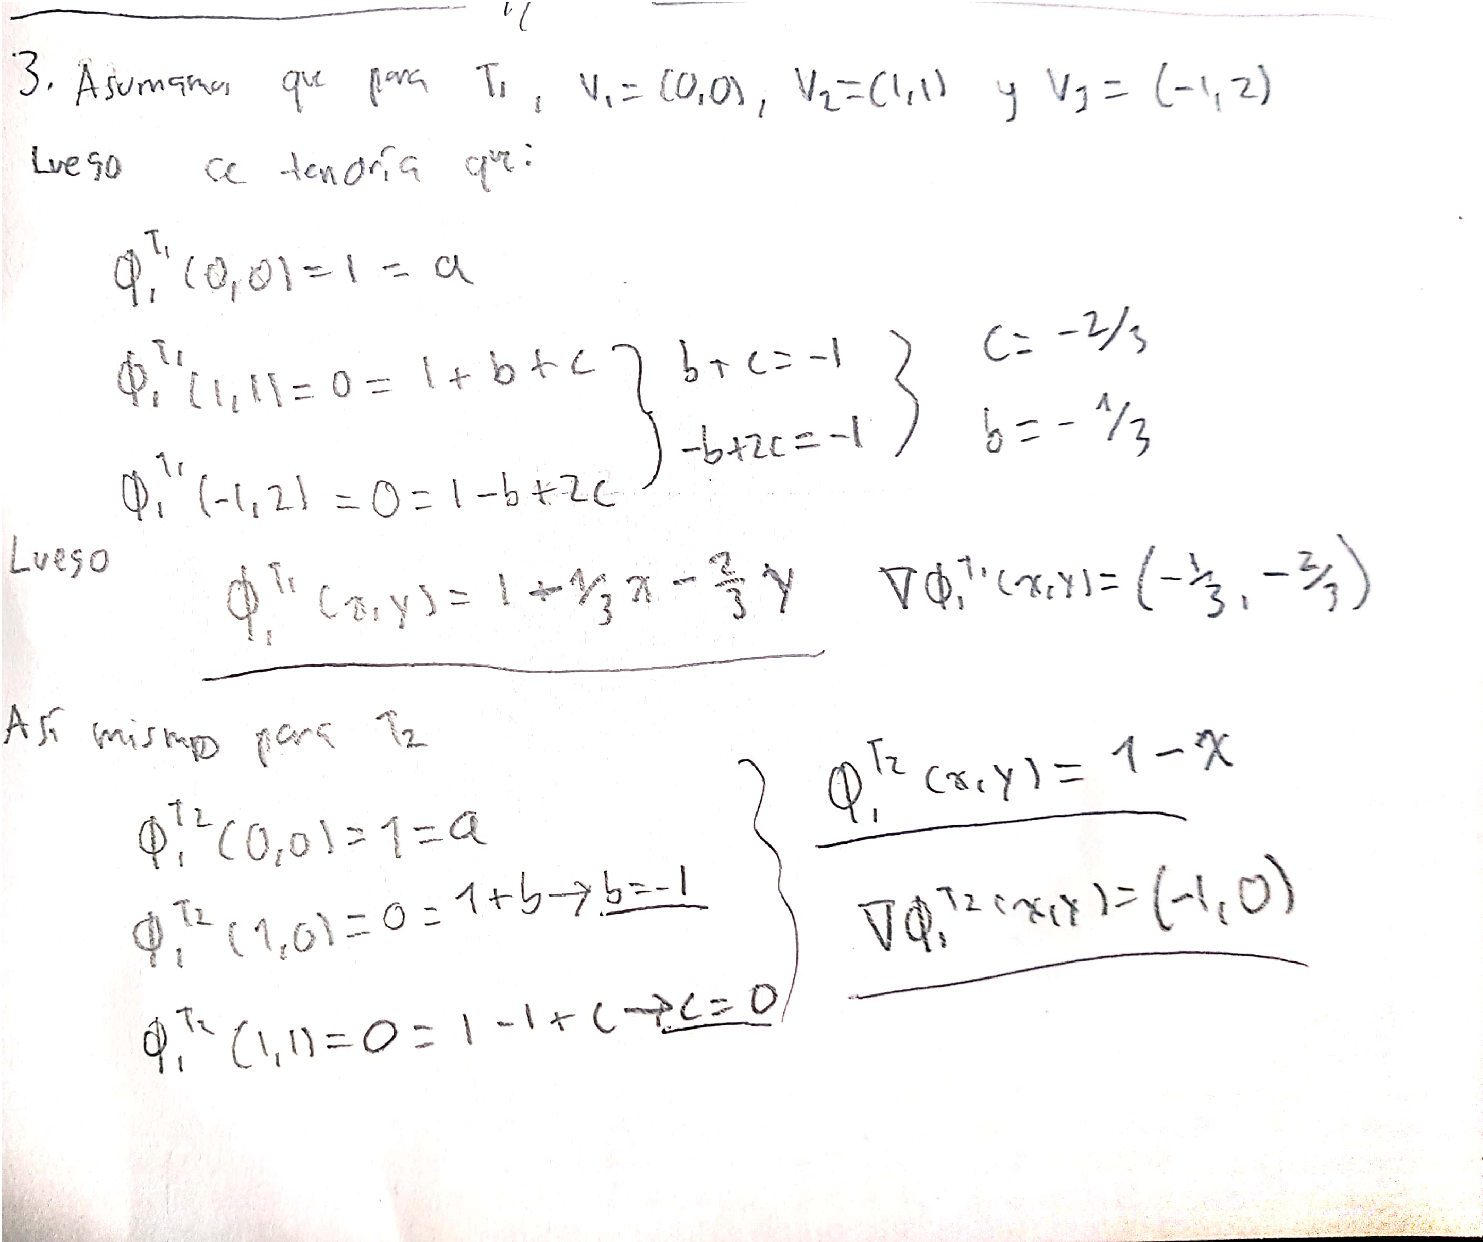
\includegraphics[scale=.4]{figs/31}
        \end{figure}
        \begin{figure}[H]
          \centering 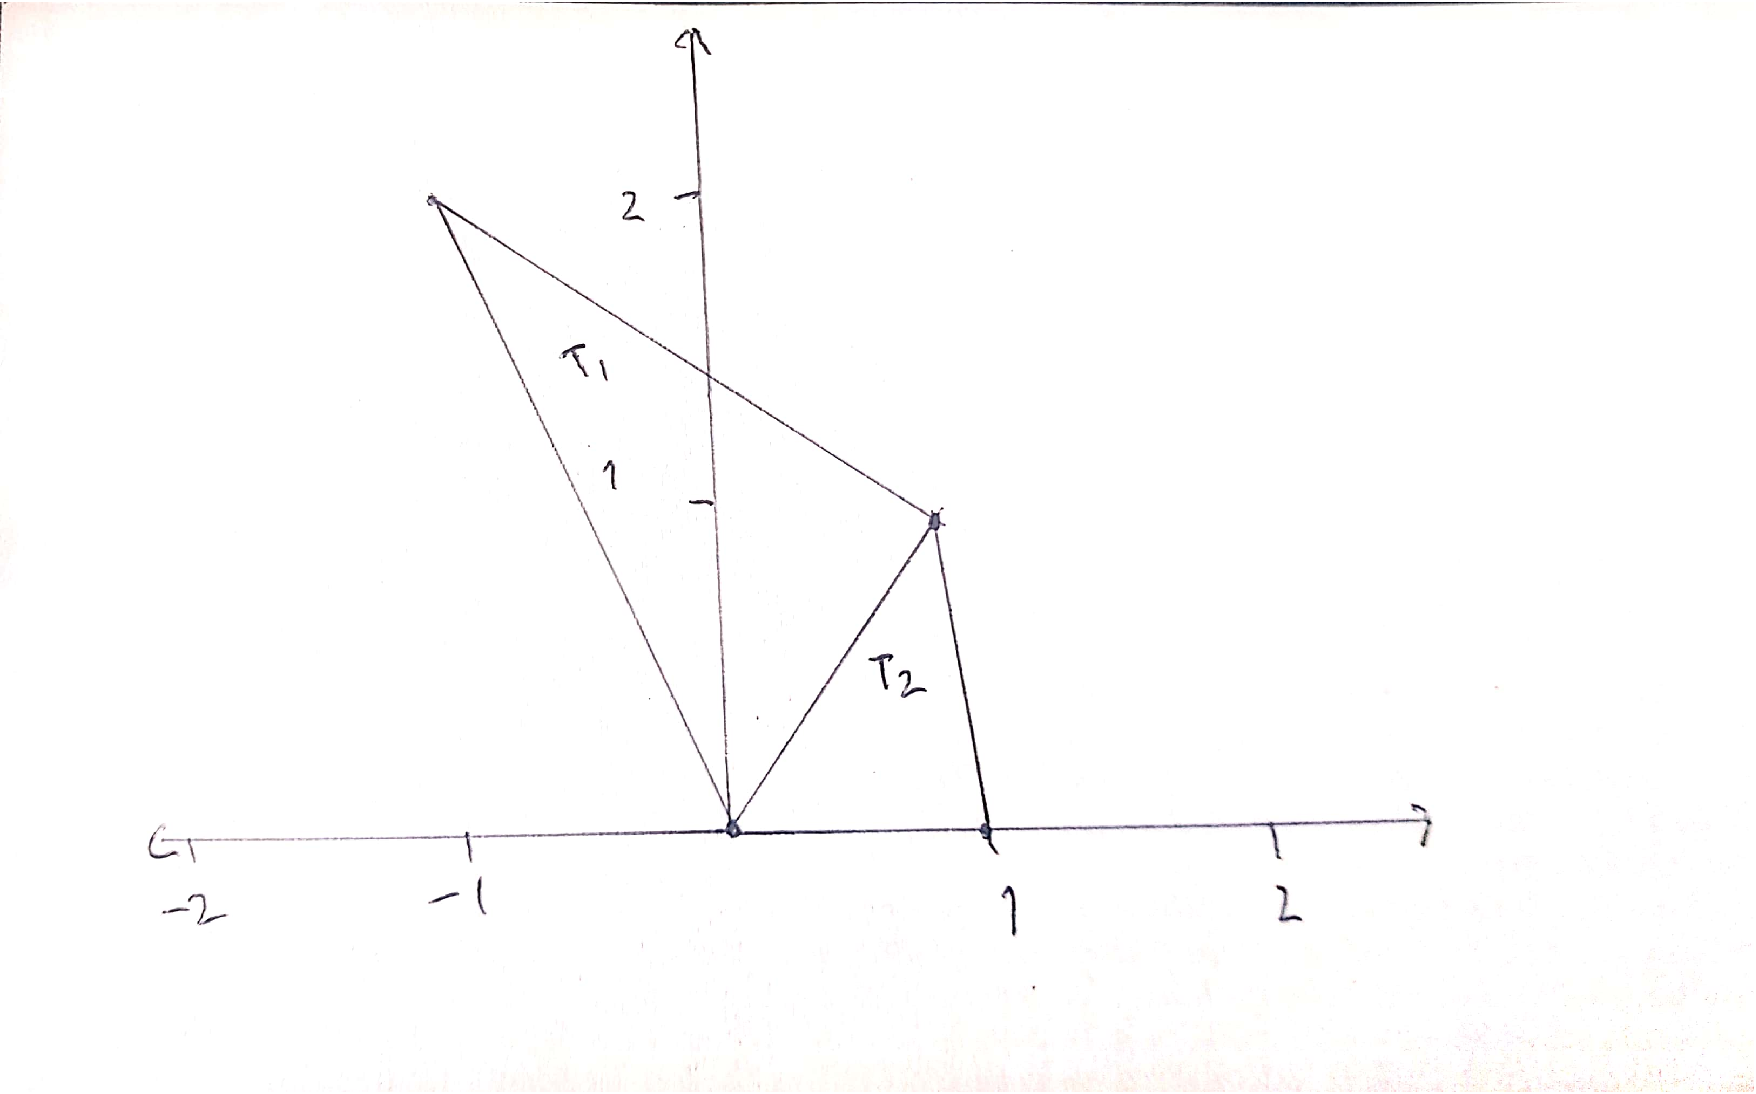
\includegraphics[scale=.4]{figs/32}
        \end{figure}
\end{enumerate}
\end{document}
